% options:
% thesis=B bachelor's thesis
% thesis=M master's thesis
% czech thesis in Czech language
% english thesis in English language
% hidelinks remove colour boxes around hyperlinks

\documentclass[thesis=B,english]{FITthesis}[2012/10/20]

% \usepackage[utf8]{inputenc} % LaTeX source encoded as UTF-8
% \usepackage[latin2]{inputenc} % LaTeX source encoded as ISO-8859-2
% \usepackage[cp1250]{inputenc} % LaTeX source encoded as Windows-1250
\usepackage{algorithm}
\usepackage{algorithmicx}
\usepackage{algpseudocode}

\usepackage{listings}

\usepackage{graphicx} %graphics files inclusion
% \usepackage{subfig} %subfigures
\usepackage{amsmath} %advanced maths
% \usepackage{amssymb} %additional math symbols

\usepackage{dirtree} %directory tree visualisation
\newtheorem{theorem}{Theorem}



% % list of acronyms
% \usepackage[acronym,nonumberlist,toc,numberedsection=autolabel]{glossaries}
% \iflanguage{czech}{\renewcommand*{\acronymname}{Seznam pou{\v z}it{\' y}ch zkratek}}{}
% \makeglossaries



% % % % % % % % % % % % % % % % % % % % % % % % % % % % % % 
% EDIT THIS
% % % % % % % % % % % % % % % % % % % % % % % % % % % % % % 

\department{Department of Computer Systems}
\title{Timing Attack on the RSA Cipher}
\authorGN{Martin} %author's given name/names
\authorFN{Andr{\' y}sek}%author's surname
\author{Martin Andr{\' y}sek} %author's name without academic degrees
\authorWithDegrees{Martin Andr{\' y}sek} %author's name with academic degrees
\supervisor{Ing. Ji{\v r}{\' i} Bu{\v c}ek}
\acknowledgements{I would like to thank to Ing. Ji{\v r}{\' i} Bu{\v c}ek for leading me in this thesis and my friends for support me during writing.}
\abstractEN{This thesis is focused on replication of timing attack on RSA cryptosystem introduced by Paul Kocher, which is done by measuring time of square and multiply algorithm with
Montgomery multiplication. The attack is based on measuring execution time of decryption function on messages with different properties. The thesis describe
main principles and vulnerabilities of RSA cryptosystem.
Implementation should be used for education purposes, mainly in security courses.}
\abstractCS{Tato pr{\' a}ce se zab{\' y}v{\' a} replikac{\' i} {\' u}toku na RSA kryptosyst{\' e}m {\v c}asov{\' y}m postrann{\' i}m kan{\' a}lem, kter{\' y} je realizov{\' a}n 
m{\v e}{\v r}en{\' i}m {\v c}asu algoritmu opakovan{\' y}ch {\v c}tvercu s Montgomeryho n{\' a}soben{\' i}m.
{\' U}tok se zame{\v r}uje na m{\v e}{\v r}en{\' i} {\v c}asu trvan{\' i} de{\v s}ifrov{\' a}n{\' i} rozd{\' i}ln{\' y}ch zpr{\' a}v s ur{\v c}it{\' y}mi vlastnostmi. Pr{\' a}ce
popisuje z{\' a}kladn{\' i} principy a slabiny RSA kryptosyst{\' e}mu. 
 V{\' y}sledkem pr{\' a}ce je demonstrativn{\' i} aplikace, kter{\' a} bude pouzita ve vyuce p{\v r}edmetech, zabyvaj{\' i}c{\' i}mi se po{\v c}{\' i}ta{\v c}ovou bezpe{\v c}nost{\' i}.
 }
\placeForDeclarationOfAuthenticity{Prague}
\keywordsCS{RSA, kryptoanal{\' y}za, {\v c}asov{\' y} {\' u}tok, postrann{\' i} kan{\' a}l, Montgomeryho n{\' a}soben{\' i} }
\keywordsEN{RSA, cryptanalysis, timing attack, side channel, Montgomery multiplication}
\declarationOfAuthenticityOption{1} %select as appropriate, according to the desired license (integer 1-6)
\website{https://github.com/vydrous/BP-code}

\begin{document}


% \newacronym{CVUT}{{\v C}VUT}{{\v C}esk{\' e} vysok{\' e} u{\v c}en{\' i} technick{\' e} v Praze}
% \newacronym{FIT}{FIT}{Fakulta informa{\v c}n{\' i}ch technologi{\' i}}
%%%%%%%%%%%%%%%%%%%%%%%%%%%%%%%%%%%%%%%%%%%%%%%%%%%%%%%%%%%%%%%%%%%%%%%%%%%%%%%%%%%%%%%%%%%%%%%%%%%%%%%%%%%%%%%%5

\setsecnumdepth{part}
\chapter{Introduction}

\paragraph*{}{
Information security is nowadays very important. Through the network flows lot of information which is essential to keep in private. Due to this, many ciphers were invented and are used to encrypt communication over network. One of these ciphers is RSA. In past time there were several vulnerabilities on this cipher. I will focus on timing attack which exploit data dependency of decrypting algorithm. 
}


\paragraph*{}
{This thesis will explain the main thoughts of RSA cryptosystem, its known vulnerabilities and how to defend against them. Thesis also introduce reader to timing attack problematic.
It will compare two targets of timing attack, Kochers original attack on multiplication versus Dhems attack on square. Although both attack can be easily defended just by eliminating
data dependency in decryption (resp. signing) algorithm.

\paragraph*{}
{
Purpose of this thesis is demonstrative. The final application should be used in cryptography courses on Faculty of Information chnologies on CTU, mainly in Advanced Cryptology course. It should demonstrate progress of guessing private key bit by bit. There will be two approaches of guessing key. First original introduced by Paul Kocher which focuses on extra modural reduction during multiply operation\cite{Kocher1996}. The second approach was introduced by J.-F. Dhem and collective where they focus on extra modular reduction during square phase\cite{Dhem}.
}

\paragraph*{}{
Lastly, I will introduce several ways of defense against timing attacks which will avoid data dependency. So that execution of time will be either constant or not telling us any usable information.
}


%%%%%%%%%%%%%%%%%%%%%%%%%%%%%%%%%%%%%%%%%%%%%%%%%%%%%%%%%%%%%%%%%%%%%%%%%%%%%%%%%%%%%%%%%%%%%%%%%%%%%%%%%%%%%%%%5

\setsecnumdepth{all}
\pagestyle{ruled}
\chapter{State-of-the-art}
\paragraph*{}{
In 1996 Paul Kocher presented timing attack on several cryptosystems including RSA\cite{Kocher1996}. The cryptosystems have in common that all of them are using modular exponentiation or they are public key cryptosystems. Kochers idea was to attack square and multiply algorithm which uses Montgomery multiplication. He intend to exploit execution time of decrypting and signing algorithms because there is dependency on private exponent. After Kocher there have been more tries with better success, for example J.-F. Dhem, F. Koeune, P.-A. Leroux, P. Mestre, J.-J. Quisquater and J.-L. Willems who improved Kochers study\cite{Dhem}.}


\paragraph*{}{
%We should decide what is the optimal amount of messages. It should not be too many so that we can guess the key in reasonable time but it have to be enough to guess the key.
}
\paragraph*{}{
%Next, we should create some defensive mechanism in cryptosystem in order to make attack fail.
}

%%%%%%%%%%%%%%%%%%%%%%%%%%%%%%%%%%%%%%%%%%%%%%%%%%%%%%%%%%%%%%%%%%%%%%%%%%%%%%%%%%%%%%%%%%%%%%%%%%%%%%%%%%%%%%%%5
\chapter{Used mathematical principles}
\paragraph*{}{
In this chapter I will introduce mathematical theorems and principles which will be referenced through the thesis
}

%%%%%%%%%%%%%%%%%%%%%%%%%%%%%%%%%%%%%%%%%%%%%%%%%%%%%%%%%%%%%%%%%%%%%%%%%%%%%%%%%%%%%%%%%%%%%%%%%%%%%%%%%%%%%%%%5
\section{Fermat's little theorem}
\theorem{(Fermat).}
{
For prime p and any \(a \in Z\) such that \(a \not\equiv 0 \pmod p,\)}

\[a^{p-1} \equiv 1 \pmod p\]
}
\paragraph*{}
{Fermat's little theorem is restricted only on prime numbers so that we will need to extende it to all integers. For that we will use Euler's theorem}
% {
% If we want to extend Fermat's little theorem to a composite modulus, a false generalization
% would be: if \(a \not\equiv 0 \pmod m\) then \(a^{m-1} \equiv 1 \pmod m\). For a counterexample, take \(m = 15\) and
% \(a = 2: 2^{14} \equiv 4 \not\equiv 1 \pmod {15}.\)}
% \paragraph*{}{
% A correct extension of Fermat's little theorem to non-prime moduli requires a new way
% of thinking about the hypothesis in Fermat's little theorem. For prime p,}
% 
% \[a \not\equiv 0 \pmod p \Longleftrightarrow (a, p) = 1,\]
% but these two conditions are not equivalent when p is replaced with a composite number.
% It is the relative primality point of view on the right that lets Fermat's little theorem be
% extended to a general modulus, as Euler discovered.
% }
%%%%%%%%%%%%%%%%%%%%%%%%%%%%%%%%%%%%%%%%%%%%%%%%%%%%%%%%%%%%%%%%%%%%%%%%%%%%%%%%%%%%%%%%%%%%%%%%%%%%%%%%%%%%%%%%5

\section{Euler's theorem}

\theorem{(Euler).}{
For \(m \ge 2 \in Z^+\) and any \(a \in Z\) such that \(\gcd(a, m) = 1\)
}
\[  a^{\phi(n)} \equiv 1 \pmod n\]
{
where \(\phi(m)\) is the number of invertible integers modulo m.

}





%%%%%%%%%%%%%%%%%%%%%%%%%%%%%%%%%%%%%%%%%%%%%%%%%%%%%%%%%%%%%%%%%%%%%%%%%%%%%%%%%%%%%%%%%%%%%%%%%%%%%%%%%%%%%%%%5

\chapter{RSA}

\paragraph*{}
{RSA is public-key cryptosystem which was developed at MIT by Ron Rivest, Adi Shamir and Leonard Adleman. The cryptosystem was published in the 1977.
}

\paragraph*{}{
%Public-key cryptosystem is ...
Main thought of public-key cryptosystem is sharing encryption key to whoever asks for it. Beacause it is used just for encryption, we can be sure that attacker could not retrieve any information about secret decryption key. Each subject of the conversation keeps his decryption key in private.
}


%%%%%%%%%%%%%%%%%%%%%%%%%%%%%%%%%%%%%%%%%%%%%%%%%%%%%%%%%%%%%%%%%%%%%%%%%%%%%%%%%%%%%%%%%%%%%%%%%%%%%%%%%%%%%%%%5

\section{Principle}
\paragraph*{}
{RSA is based on modular exponentiation. There is three important numbers which are used in computing modular exponation resp. crypting messages.}
\begin{itemize}
 \item \(n\) - Modulus which is used during whole cipher algorith.
 \item \(e\) - Encryption exponent. Exponent \(e\) is used to modular exponation of message so that we get ciphertext. Exponent must meet the condition  \(\gcd(e,\phi(n)) = 1\) where \(\phi\) is Euler's totient function and \(gcd\) is the greatest common divider function. This condition will be explained later.
 \item \(d\) - Decryption exponent. It is computed by finding modular inversion of public exponet \(e\) in modulus \(\phi(n)\).
\end{itemize}
{Commonly used value of \(e\) is 65537.}
\paragraph*{}
{The cryprosystem consist of two keys, public and privat. Public key is used for encrypting messages and is composed of modulus \(n\) and public exponet \(e\). Private key is composed of modulus \(n\) and private exponent \(d\)

\begin{figure}
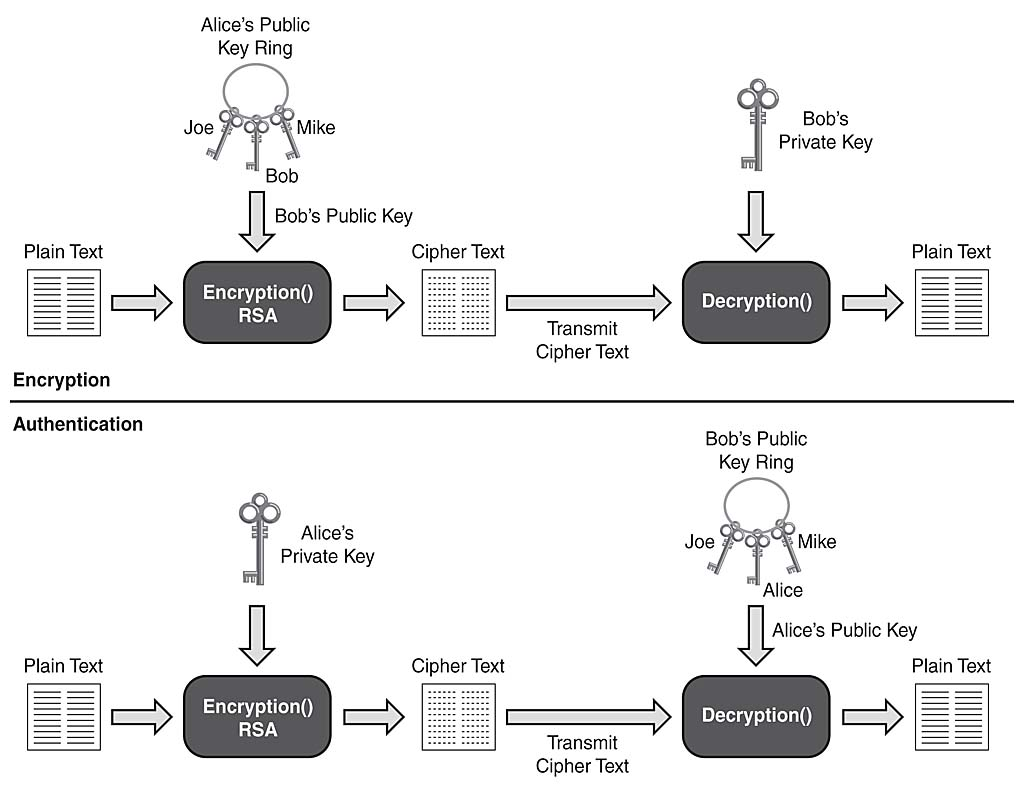
\includegraphics[scale=0.3]{rsa-principle.jpg}
\caption{RSA illustration\cite{img1}
} 
\end{figure}

}



%%%%%%%%%%%%%%%%%%%%%%%%%%%%%%%%%%%%%%%%%%%%%%%%%%%%%%%%%%%%%%%%%%%%%%%%%%%%%%%%%%%%%%%%%%%%%%%%%%%%%%%%%%%%%%%%5


\subsection{Key generation}
\paragraph*{}
{This is steps needed to generate keypair including public and private key}
\begin{itemize}
 \item Generate \(p\) and \(q\), which have to be distinct prime numbers large enough to make factorization of their product hard problem. If we choose too small \(p\) and \(q\), we are risking that attacker could do factorization of \(n\) so that he could easily compute our private exponent \(d\) using Euler's totient function \(\phi\).
 \item Compute \(n\), where \(n = p  q\)
 \item Compute Euler's totient function \(\phi(n)\). Because we know \(p\) and \(q\) it is simple to compute it. We know that  \(n\) is product of \(p\) and \(q\) which are prime numbers. Euler's totient function \(\phi\) for prime numers equals \(\phi(P) = P -1\) where \(P\) is prime number. Also we know that Euler's totient function \(\phi\) is multiplicative. So the problem is:
 \[\phi(n) = \phi(p*q)\]
 Now we use multiplicative rule:
 \[\phi(p*q)\ = \phi(p)* \phi(q) = (p - 1)(q - 1)\]
 Then we get simple formula for comupting \(\phi(n)\)
 \[\phi(n) = (p - 1)(q - 1)\]
 \item Generate \(e\) from 3 to  \(n - 1\) which meets condition \(\gcd(e,\phi(n)) = 1\). In most implementation of RSA is used \(e = 65537 = 2^{16} + 1\)
 \item Compute \(d = e^{-1}\bmod{\phi(n)} \)
 \item The pair \((e,n)\) is released as public key
 \item The pair \((d,n)\) is kept secret as private key
\end{itemize}
%%%%%%%%%%%%%%%%%%%%%%%%%%%%%%%%%%%%%%%%%%%%%%%%%%%%%%%%%%%%%%%%%%%%%%%%%%%%%%%%%%%%%%%%%%%%%%%%%%%%%%%%%%%%%%%%5

\subsection{Key distribution}
\begin{itemize}
 \item Alice would like to send Bob secret message.
 \item Bob generates public key \((e,n)\) and his private key \((d,n)\).
 \item Bob sends Alice public key using reliable route (it has not to be secret route).
 \item Due to high value of \(n\) possible attacker will not be able compute \(d\) from public keypair \((e,n)\) because factorization of \(n\) is not possible in polynomial time.
 \item Alice uses it to encrypt her message and sends it to Bob. 
 \item Bob decrypts her message using his private key.
\end{itemize}
 %would like to send Bob secret message. Bob generates public key \((e,n)\) and his private key \((d,n)\). Bob sends Alice public key using reliable route (it has not to be secret route). Due to high value of \(n\) possible attacker will not be able compute \(d\) from public keypair \((e,n)\) because factorization of \(n\) is not possible in polynomial time. Alice uses it to encrypt her message and sends it to Bob. Bob decrypts her message using his private key.}
%%%%%%%%%%%%%%%%%%%%%%%%%%%%%%%%%%%%%%%%%%%%%%%%%%%%%%%%%%%%%%%%%%%%%%%%%%%%%%%%%%%%%%%%%%%%%%%%%%%%%%%%%%%%%%%%5

\subsection{Encryption}
\paragraph*{}
{Encryption is done by using public keypair \((e, n)\): \[c = | m^e | _n\]
where \(m\) is plaintext message and \(c\) is encrypted message which will be sent to receiver.
}
%%%%%%%%%%%%%%%%%%%%%%%%%%%%%%%%%%%%%%%%%%%%%%%%%%%%%%%%%%%%%%%%%%%%%%%%%%%%%%%%%%%%%%%%%%%%%%%%%%%%%%%%%%%%%%%%5

\subsection{Decryption}
\paragraph*{}
{Decryption is done similar thanks to relation \(ed \equiv 1 \pmod{\phi(n)}\). We can simply power ciphertext to our private exponent \(d\) to obtain original message.  
\[ |c^d|_n = |(m^e)^d|_n = | m^{ed}|_n \]

Now that we know, that \(ed \equiv 1 \pmod{\phi(n)}\) which can be overwriten to form \(ed = 1 + k*\phi(n)\). From that we get:
\[| m^{ed}|_n = | m^{1+ k*\phi(n) }|_n = | m^1 * m^{ k*\phi(n)}|_n\]

From Euler's theorem (\(a^{\phi(n)} \equiv 1 \pmod{n}\)) we can substitute \(m^{ k*\phi(n)}\) for 1.


\[| m^1 * m^{ k*\phi(n)}|_n = | m^1 * 1|_n =  m\]

We got desired message \(m\). 
}
%%%%%%%%%%%%%%%%%%%%%%%%%%%%%%%%%%%%%%%%%%%%%%%%%%%%%%%%%%%%%%%%%%%%%%%%%%%%%%%%%%%%%%%%%%%%%%%%%%%%%%%%%%%%%%%%5

\subsection{Signing}
\paragraph*{}{
RSA signing is used to verify wheter the message was not changed on the way from sender to reciever. The process is really similar to decryption but we do not encrypt message itself. We first use some one way function on message, mostly there is used some hash function, then we encrypt the hash of the message but we use our private exponent for encryption. That would mean anyone could decrypt the signature by using our public key and compare it with actual has of the recieved message. If they equals we can be sure that it is original message and was not changed on the way to from sender. If someone tries to change the content of message, he has to have sender private key to generate valid signature, otherwise he will not be able to generate signature from different hash (which has to change, when he change the content of message).

}
%%%%%%%%%%%%%%%%%%%%%%%%%%%%%%%%%%%%%%%%%%%%%%%%%%%%%%%%%%%%%%%%%%%%%%%%%%%%%%%%%%%%%%%%%%%%%%%%%%%%%%%%%%%%%%%%5
\section{Security}

\paragraph*{}{
Security of RSA is relied on inability to do factorization of large integer in polynomial time. From paper ``Factoring estimates for a 1024-bit RSA modulus''\cite{} we can say that breaking 1024-bit RSA key would last about year long on device worth of 10 milions american dolars.
}

\paragraph*{}{
There is a community challenge where people trying to factorize RSA keys of different length. The latest succces was on 768-bit length key which was factored in 2009. In that time the facotrization took 3 years of execution time. Nowadays standart key length is 1024 which have not been factored yet.
}

%%%%%%%%%%%%%%%%%%%%%%%%%%%%%%%%%%%%%%%%%%%%%%%%%%%%%%%%%%%%%%%%%%%%%%%%%%%%%%%%%%%%%%%%%%%%%%%%%%%%%%%%%%%%%%%%5

\section{Optimization}
\paragraph*{}
{Because we generally use high value of modulus \(n\) the exponentiation of message of similar bit length is quite time consuming so several algorithms to increase speed of computation was developed.}
%%%%%%%%%%%%%%%%%%%%%%%%%%%%%%%%%%%%%%%%%%%%%%%%%%%%%%%%%%%%%%%%%%%%%%%%%%%%%%%%%%%%%%%%%%%%%%%%%%%%%%%%%%%%%%%%5

\subsection{Chinese remainder theorem}

\paragraph*{}
{By using CRT we can significantly speed up decryption of received messages or signing outcoming message. This method is not usable during encrypting phase because we need to know \(p\) and \(q\) factors of \(n\) which are parts of private key.
Assuming that \(p>q\) we can divide :}

\[dP = e^{-1} \pmod{p-1}\]
\[dQ = e^{-1} \pmod{q-1}\]
\[qInv = q^{-1} \pmod{p}\]

\paragraph*{}
{After that, we compute message \(m\) with given c:}

\[m_1 = c^{dP} \pmod{p}\]
\[m_2 = c^{dQ} \pmod{q}\]
\[h = qInv \cdot (m_1 - m_2) \pmod{p}\]  
\[m = m_2 + hq\]

\paragraph*{}
{Finding modular exponentiation cost grows with cube of number of the bits in \(n\), so it is still more efficient to do two exponentiation with half sized modulus}


%%%%%%%%%%%%%%%%%%%%%%%%%%%%%%%%%%%%%%%%%%%%%%%%%%%%%%%%%%%%%%%%%%%%%%%%%%%%%%%%%%%%%%%%%%%%%%%%%%%%%%%%%%%%%%%%5

\subsection{Montgomery Multiplication}

\paragraph*{}
{Normal modular multiplication could be quite slow for large numbers, due to processor have to run several operations before it gets desired remainder. On the other hand P. L. Montgomery developed algorithm which assumes that processor do division by power of 2 really fast.}
\paragraph*{}{
Montgomery presented algorithm, which transform numbers to Montgomery base and then compute modular multiplication efficiently. To transform number to Montgomery base we need to compute \(\bar{a} = ar \pmod{n}\) where \(r\) is the next  power of 2 greater than \(n\). For example if \(2^{63} < n < 2^{64}\) then desired \(r\) will be \(2^{64}\). The multiplication in Montgomery base is done by: \[\bar{u} = \bar{a}\bar{b}r^{-1} \pmod{n}\] where \(r^{-1}\) is modular inversion of \(r\).
}
\paragraph*{}{
As we can see \(\bar{u}\) is in Montgomery base of the corresponding 
\(u = ab \pmod{n}\) 
since}

\begin{equation}
\begin{split}
\bar{u} & = \bar{a}\bar{b}r^{-1} \pmod{n} \\
 & = (ar)(br)r^{-1} \pmod{n} \\
 & = (ab)r \pmod{n}
\end{split}
\end{equation}
\medskip

\paragraph*{}{
Montgomery reduction which gives us \(\bar{u}\) is implemented this way:
}

\begin{algorithm}[H]
\alglanguage{pseudocode}
\caption{Montgomery Reduction}
\begin{algorithmic}[1]
\Function{Mon\_Red}{$\bar{a},\bar{b}, N$}
 \State $t \gets\bar{a} *\bar{b}$
 \State $m \gets N^{-1} * t \pmod{r}$
 \State $\bar{u} \gets (t + mN) / r$
 \If {$\bar{u}>N$}
  \State $\bar{u} \gets\bar{u} - N$
 \EndIf
\State \textbf{return} $\bar{u}$
\EndFunction
\end{algorithmic}
\end{algorithm}

\paragraph*{}
{
Its main advance is that it never performs division by the modulus \(n\) but we still need to find out \(u\) and precompute \(n^{-1}\) using the extended Euclidean algorithm.
It is done by this algorithm: }

\begin{algorithm}[H]
\caption{Montgomery Multiplication}
\begin{algorithmic}[1]
\Function{Mon\_Mult}{$a,b, n$}
 \State $r \gets 2^{BitLen(n)}$
 \State \textit{Compute \(n^{-1}\) using the extended Euclidean algorithm}
 \State $\bar{a} \gets a *r \pmod{n}$
 \State $\bar{b} \gets b * r \pmod{n}$
 \State $\bar{u} \gets Mon\_Red(\bar{a}, \bar{b})$
 \State $u \gets Mon\_Red(\bar{u}, 1)$
 \State \textbf{return} $u$
\EndFunction
\end{algorithmic}
\end{algorithm}

%%%%%%%%%%%%%%%%%%%%%%%%%%%%%%%%%%%%%%%%%%%%%%%%%%%%%%%%%%%%%%%%%%%%%%%%%%%%%%%%%%%%%%%%%%%%%%%%%%%%%%%%%%%%%%%%5

\subsection{Square and Multiply}
\paragraph*{}
{This optimization uses bitwise representation of the exponent. The algorithm picks all byte from left (MSB) to right and despite their value, 
it determines which operation will be performed for each bit. For bits equal to 1 we perform squaring preset value \(c\) then we multiply it with the base of exponentiation \(m\). 
For bits equal to 0 we just perform squaring part. Therefore we get data dependent operation, which will be used in our attack. For even faster implementation we use Montgomery
multiplication instead of normal one. In some papers this Square and Multiply algorithm is called Montgomery exponentiation}



\begin{algorithm}[H]
\caption{Square \& Multiply algorithm}
\begin{algorithmic}[1]
\Function{Square\_and\_Multiply}{$m,e,n$}
 \State $c\gets 1$
 \State $k\gets BitLen(e)$
 \For {$i \gets k-1, \, 0$}
  \State $c \gets Mon\_Mult(c,c)$
  \If {$e[i] == 1$}\Comment{\(i\)th bit of exponent \(e\) }
   \State $c \gets Mon\_Mult(c,m)$
  \EndIf
 \EndFor
\State \textbf{return} $c$
\EndFunction
 
\end{algorithmic}
\end{algorithm}

%%%%%%%%%%%%%%%%%%%%%%%%%%%%%%%%%%%%%%%%%%%%%%%%%%%%%%%%%%%%%%%%%%%%%%%%%%%%%%%%%%%%%%%%%%%%%%%%%%%%%%%%%%%%%%%%5
\section{Vulnerabilities}
\paragraph*{}
{TODO}


\chapter{Attacks}
\paragraph*{}{
The basic idea of timing attacks was presented by Kocher in 1996. He specified theoretical attacks not only on RSA.
}

\paragraph*{}{
Both variant of attack are based on similar principle. They divide messages from set \(M\) to several subsets \(M_i\) due to response of some Oracle \(O\). Then by measuring time of decrypting or signing and 
guessing bits of secret exponent by comparing times of each set.
}
%%%%%%%%%%%%%%%%%%%%%%%%%%%%%%%%%%%%%%%%%%%%%%%%%%%%%%%%%%%%%%%%%%%%%%%%%%%%%%%%%%%%%%%%%%%%%%%%%%%%%%%%%%%%%%%%5

\section{Attack on multiply}
\paragraph*{}{
First Kochers idea was to exploit multiply operation in Square and Multiply algorithm. Kocher mean to measure time of decryption (or signing) messages using the private key \(d\) 
and focus on conditional multiply step. We are attacking each bit of \(d\) with knowledge of \( i-1\) bits we can guess the \(i\)th bit. Let \(d = d_1,d_2, \ldots ,d_k \) where \(k\) is bit length of \(d\) and \(d_1\) is MSB. 
We can assume that \( d_1 = 1\) so we can attack bit \(d_2\).
}
\paragraph*{}{
We need oracle \(O\) which predict whether final Montgomery reduction happened during multiply step:
}
\paragraph*{}

\( O(m) =\) $\left\{
  \begin{array}{cl}
    \text{1} & \text{\mbox{if}  \(m^2 * m\) is done with final reduction} \\
    \text{0} & \text{\mbox{if}  \(m^2 * m\) is done without final reduction} 
  \end{array}
\right.$

\paragraph*{}
{
where \(m\) is message from set \(M\). We can now divide messages to 2 subsets:}

\[M_1 = \{m \in M : O(m) = 1\}\]
\[M_2 = \{m \in M : O(m) = 0\}\]

\paragraph*{}{
We can now measure time of these two subsets. We are expecting same times for doing square part, but in multiply part will be messages from \(M_1\) higher, due to
final Montgomery Reduction. We compare means of sets \(M_1\) and \(M_2\). If time of \(M_1\) is significantly bigger then the final reduction was done therefore bit \(d_2\)
is 1. If the times of \(M_1\) and \(M_2\) are equal then bit \(d_2\) is 0. . }

\paragraph*{Problem:}{
We cannot be sure what is significant difference between time means. So our guesses cannot be precise.}
%%%%%%%%%%%%%%%%%%%%%%%%%%%%%%%%%%%%%%%%%%%%%%%%%%%%%%%%%%%%%%%%%%%%%%%%%%%%%%%%%%%%%%%%%%%%%%%%%%%%%%%%%%%%%%%%5

\section{Attack on square}
\paragraph*{}{
Focusing on squaring operation will give us better results. The procedure is similar but we generate two oracles and four sets of messages. We similarly iterate
through the bits of secret key \(d\) as in multiply attack. When we know \( i - 1 \) bits and we are guessing \(i\)th bit we compute \(m_{temp}\) 
which has value before unknown possible multiplication step.\cite{Dhem}
}
\paragraph*{}{
We first presume that bit \(d_i\) is 1. If the presumption is right then the following steps will be executed. \(m_{temp}\) will be multiplied by \(m\), 
then the result of multiplication will be squared. We will execute the multiplication step and then we will check if in the square step is done with or without reduction.
By this criterion we divide messages to subsets \(M_1\) if the reduction was computed or \(M_2\) if not. The oracle will be:
}
\paragraph*{}
\( O_1(m) =\) $\left\{
  \begin{array}{cl}
    \text{1} & \text{\mbox{if}  \((m_{temp} * m)^2\) is done with final reduction} \\
    \text{0} & \text{\mbox{if}  \((m_{temp} * m)^2\) is done without final reduction} 
  \end{array}
\right.$
\paragraph*{}{
Secondly, we presume that bit \(d_i\) is 0. In that case only the square phase \(m_{temp}^2\) will be executed so we similarly divide messages to subsets \(M_3\) with reduction and 
\(M_4\) without reduction. Oracle \(O_2\):
}


\paragraph*{}
\( O_2(m) =\) $\left\{
  \begin{array}{cl}
    \text{1} & \text{\mbox{if}  \(m_{temp}^2\) is done with final reduction} \\
    \text{0} & \text{\mbox{if}  \(m_{temp}^2\) is done without final reduction} 
  \end{array}
\right.$

\paragraph*{}{
We now get 4 subsets of \(M\):
}
\paragraph*{}
\[M_1 = \{m \in M : O_1(m) = 1\}\]
\[M_2 = \{m \in M : O_1(m) = 0\}\]
\[M_3 = \{m \in M : O_2(m) = 1\}\]
\[M_4 = \{m \in M : O_2(m) = 0\}\]

\paragraph*{}
{Let \(T_i(M_i)\) be the mean time of computing messages from \(M_i\). }


\paragraph*{}{
Certainly, only one of oracles is giving us the right results. We can compare time difference between \( O_1 \) and \(O_2\). That means if \(T_1 - T_2 \) is greater than 
\(T_3 - T_4\) then we can be sure that bit \(d_i\) is 1, otherwise \(d-i\) is 0. The problem from multiply attack is no more actual because one of the differences have to be higher
than other.
}
%%%%%%%%%%%%%%%%%%%%%%%%%%%%%%%%%%%%%%%%%%%%%%%%%%%%%%%%%%%%%%%%%%%%%%%%%%%%%%%%%%%%%%%%%%%%%%%%%%%%%%%%%%%%%%%%5


\chapter{Defense}
\section{Additional reduction}
\paragraph*{}{
The most obvious defense is to add dummy subtraction to Montgomery reduction algorithm which does not change any value but consume the same amount of time as if the real subtraction
was performed. This should not significantly slow the computation but it totally eliminate this type of timing attack by making Montgomery reduction constant time function.
}
%%%%%%%%%%%%%%%%%%%%%%%%%%%%%%%%%%%%%%%%%%%%%%%%%%%%%%%%%%%%%%%%%%%%%%%%%%%%%%%%%%%%%%%%%%%%%%%%%%%%%%%%%%%%%%%%5

\section{Masking}
\paragraph*{}{
We can mask the ciphertext before computation of \(c^d \pmod{n}\) so the attacker will not know which cipher text is decrypted. It is done simply by generating pair of masks 
before each exponentiation. We generate random mask \(m\). Then we compute \(m'\):
\[ m' = (m^{-1})^e \pmod{n}\]
where \(e\) is public exponent.
}
\paragraph*{}
{Before each exponentiation we multiply the ciphertext \(c\) with mask \(m'\) so we get masked \(x_m\):
\begin{equation}
\begin{split}
 x_m & = (c*m')^d \pmod{n} \\
 & = (c * (m^{-1})^e)^d \pmod{n}  \\
 & = c^d * m^{-1} \pmod{n}
\end{split}
\end{equation}
from where we can see that \(c^d\) is our desired message masked by \(m^{-1}\). Then we simply recover \(x\) by multiplying by \(m\)\cite{Kocher1996}:
\begin{equation}
\begin{split}
 x & = x_m * m \pmod{n} \\
 & = x * m^{-1} * m \pmod{n}  \\
 & = x \pmod{n}
\end{split}
\end{equation}
}

\paragraph*{}{
To avoid situation when even generating of mask could become target of timing attack, there is simple workaround. To generate new mask, just square the mask pair:\cite{Kocher1996}
\[m = m^2 \pmod{n}\]
\[m' = m'^2 \pmod{n}\]

}
%%%%%%%%%%%%%%%%%%%%%%%%%%%%%%%%%%%%%%%%%%%%%%%%%%%%%%%%%%%%%%%%%%%%%%%%%%%%%%%%%%%%%%%%%%%%%%%%%%%%%%%%%%%%%%%%5

\chapter{Realisation}
%%%%%%%%%%%%%%%%%%%%%%%%%%%%%%%%%%%%%%%%%%%%%%%%%%%%%%%%%%%%%%%%%%%%%%%%%%%%%%%%%%%%%%%%%%%%%%%%%%%%%%%%%%%%%%%%5

\section{RSA implementation}

\paragraph*{}{
For our purposes we cannot use existing RSA implementation because they commonly have this vulnerability fixed. So it was needed to write own unsecure implementation of RSA cryptosystem.
It is still possible use key generation algorithm from OpenSSL because it is not target of our attack. Python 3.6.1 was used and module Crypto for working with keys.
}
%%%%%%%%%%%%%%%%%%%%%%%%%%%%%%%%%%%%%%%%%%%%%%%%%%%%%%%%%%%%%%%%%%%%%%%%%%%%%%%%%%%%%%%%%%%%%%%%%%%%%%%%%%%%%%%%5
\subsection{Montgomery}{
The main part of RSA is mechanism for modular exponentiation. As was told before we are using Montgomery multiplication for speed up computation. It is based on pseudocode in section 2.2.2.
}
\paragraph*{}
\begin{lstlisting}[language=Python]
def montgomery_product(a, b, n, r, n_inv):
    t = (a * b)
    m = ((t & (r - 1)) * n_inv) & (r - 1)
    u = (t + m * n) >> (r.bit_length() - 1)
    if u > n:
        return u - n
    return u
\end{lstlisting}

\paragraph*{}{
Some optimization was done to let reduction have greater time impact. Instead of modulo \(r\) is used bitwise AND with \(r-1\) and instead of division by \(r\) is used bitwise
shift to right \(r.bit\_length() - 1\).
}
%%%%%%%%%%%%%%%%%%%%%%%%%%%%%%%%%%%%%%%%%%%%%%%%%%%%%%%%%%%%%%%%%%%%%%%%%%%%%%%%%%%%%%%%%%%%%%%%%%%%%%%%%%%%%%%%5

\subsection{Square and Multiply}{
Due to computation in Montgomery base we also need to little edit the square and multiply algorithm to transform arguments to Montgomery base and at the end back to normal base.
We also need precompute \(r\) and \(n^{-1}\).
}

\begin{lstlisting}[language=Python]
 def square_and_multiply(ot, n, e):
    r = 2 ** (n.bit_length())
    g, n_inv, r_inv = egcd(n, r)

    if (r * r_inv + n * n_inv) == 1:
        n_inv = -n_inv % r
    else:
        raise Exception("bad GCD")

    ot = (ot * r) % n
    st = (1 * r) % n
    for i in "{0:b}".format(int(e)):
        st = montgomery_product(st, st, n, r, n_inv)
        if i == '1':
            st = montgomery_product(st, ot, n, r, n_inv)
    return montgomery_product(st, 1, n, r, n_inv)
\end{lstlisting}
%%%%%%%%%%%%%%%%%%%%%%%%%%%%%%%%%%%%%%%%%%%%%%%%%%%%%%%%%%%%%%%%%%%%%%%%%%%%%%%%%%%%%%%%%%%%%%%%%%%%%%%%%%%%%%%%5

\subsection{Encryption and decryption}{
Encryption and decryption are done just by loading keys from .pem file, then passing them to square\_and\_multiply function
}
\newpage
\section{Attack implementation}
%%%%%%%%%%%%%%%%%%%%%%%%%%%%%%%%%%%%%%%%%%%%%%%%%%%%%%%%%%%%%%%%%%%%%%%%%%%%%%%%%%%%%%%%%%%%%%%%%%%%%%%%%%%%%%%%5

\subsection{Generating and sorting messages}
\paragraph*{}{ 
For both types of attack we are starting with set of randomly generated messages. We give them to oracle which tell us which subset message belongs to. Python module \(timeit\) is used for time measurements. This chunk of code assign times to messages:
}
\paragraph*{}
\begin{lstlisting}[language=Python]
import timeit

message_times = dict()
message_range = 50000

for i in range(0, message_range):
    tmp = random.randint(0, n)

    t = timeit.Timer('decrypt.decrypt(int(m1))', 
	      setup='import decrypt; m1 = %i' % tmp)

    r = t.timeit(1)

    message_times[tmp] = r
\end{lstlisting}

%%%%%%%%%%%%%%%%%%%%%%%%%%%%%%%%%%%%%%%%%%%%%%%%%%%%%%%%%%%%%%%%%%%%%%%%%%%%%%%%%%%%%%%%%%%%%%%%%%%%%%%%%%%%%%%%5

\subsubsection{Multiply}
\paragraph*{}{
In this version we are attacking multiply operation. We use oracle which is very similar to RSA square\_and\_multiply function only with one difference.
When the final reduction is processed, function return not only result of exponentiation but also bit which tell us that the reduction have been done.}

\begin{lstlisting}[language=Python]
  ...
  if u > n:
    return u - n, 1
  return u, 0
\end{lstlisting}

\paragraph*{}
{
Based on this bit we decide in which subset the message is. The subsets are distinct. Experimentally, we can say that about one quarter of messages belongs~to
subset with reduction computed.
}
\subsubsection{Square}
\paragraph*{}{
Square attack is similar but we have two oracles which are telling us about reduction on squaring phase. Every time we give the oracle even exponent so 
multiplication phase will never be the last operation. Each of these oracles divide set of messages to two subsets which are distinct to each other. Each message 
belongs to one of \(M_1\) or \(M_2\) and to one of \(M_3\) or \(M_4\)
}
%%%%%%%%%%%%%%%%%%%%%%%%%%%%%%%%%%%%%%%%%%%%%%%%%%%%%%%%%%%%%%%%%%%%%%%%%%%%%%%%%%%%%%%%%%%%%%%%%%%%%%%%%%%%%%%%5

\subsection{Deciding the bit}

\subsubsection{Multiply}
\paragraph*{}{
We will compare mean times of the subsets of messages. If \(M_1\) is significantly greater then we set guessed bit to 1 and if they differ slightly we set the bit to 0. There is problem with telling what is significant difference because there is lot of noise. The noise is caused by other reductions done by other bits of secret key.

}
%%%%%%%%%%%%%%%%%%%%%%%%%%%%%%%%%%%%%%%%%%%%%%%%%%%%%%%%%%%%%%%%%%%%%%%%%%%%%%%%%%%%%%%%%%%%%%%%%%%%%%%%%%%%%%%%5

\subsubsection{Square}
\paragraph*{}{
We will compare differences between oracles. If oracle predicting multiply has greater difference between subsets we set 1, otherwise we set 0
}

\paragraph*{}
{I tested two different implementation of square attack. The difference is between oracles. One implementation has naive oracle which simply do whole square and multiply algorithm 
for each message. The second approach is to safe values of particular powers so the oracle does not need to compute whole square and multiply algorithm in each iteration. It just need
one square and optional multiplication in each step.
}

\paragraph*{}{
On the other hand, the naive implementation gives better results but is slightly slower.
}
%%%%%%%%%%%%%%%%%%%%%%%%%%%%%%%%%%%%%%%%%%%%%%%%%%%%%%%%%%%%%%%%%%%%%%%%%%%%%%%%%%%%%%%%%%%%%%%%%%%%%%%%%%%%%%%%5

\subsection{Assembling secret exponent}
\paragraph*{}{
After every guessed bit, it is added to variable d which is used by the oracles. After concatenation the new guessed exponent is tested if it is correct exponent.
The the test is:}
\begin{itemize}
 \item Pick some message from set
 \item Decrypt that message
 \item Do exponentiation of encrypted message to guessed private exponent \(d\)
\end{itemize}

\paragraph*{}{
During attack on square we are one cycle ahead so we have no option how to decide LSB so we just try to test both values of last bit.
}

\paragraph*{}
{For better fault toleration we could try guessing of last few bits by brute-force. When the whole attack is finished unsuccessfuly, we can go back few bits and try to all the possibilities of key suffix. It seems reasonable to do this with maximally last 10 bits. There will be extra 1024 encryption and decryption, but it is still more efficient then repeating whole attack.
}
%%%%%%%%%%%%%%%%%%%%%%%%%%%%%%%%%%%%%%%%%%%%%%%%%%%%%%%%%%%%%%%%%%%%%%%%%%%%%%%%%%%%%%%%%%%%%%%%%%%%%%%%%%%%%%%%5

\setsecnumdepth{part}
\chapter{Conclusion}

\paragraph*{}{
In my environment it was impossible to make any attack sufficient. Attack on multiply takes time to set the limit when the times differs. Even with sufficient coefficient and 
10 000 samples there was no more than 50\% success on guessing first unknown bit.}

\paragraph{}{
Attacking square was far more interesting. On 50 000 samples algorithm occasionally fails up to guessing 3 bits, but there are more cases when algorithm correctly guess more than 40 bits of key.		
}




\paragraph*{}{
Because attacks do not work entirely there was no need of implementing defenses in RSA implementation.
}
\bibliographystyle{iso690}
\bibliography{mybibliographyfile,Kocher}


\setsecnumdepth{all}
\appendix

\chapter{Acronyms}
% \printglossaries
\begin{description}
	\item[RSA] Rivest, Shamir, Adleman
	\item[MSB] Most significant bit
	\item[LSB] Least significant bit
	\item[CRT] Chinese remainder theorem
\end{description}


\chapter{Contents of enclosed CD}

%change appropriately

\begin{figure}
	\dirtree{%
		.1 readme.txt\DTcomment{the file with CD contents description}.
		.1 exe\DTcomment{the directory with executables}.
		.1 src\DTcomment{the directory of source codes}.
		.2 wbdcm\DTcomment{implementation sources}.
		.2 thesis\DTcomment{the directory of \LaTeX{} source codes of the thesis}.
		.1 text\DTcomment{the thesis text directory}.
		.2 thesis.pdf\DTcomment{the thesis text in PDF format}.
		.2 thesis.ps\DTcomment{the thesis text in PS format}.
	}
\end{figure}

\end{document}
